\chapter{System Study}

The system study phase involves analysing existing educational platforms, identifying operational limitations, surveying foundational literature, defining the architecture of the proposed system, and establishing the technical requirements for development. The study provides the rationale for replacing conventional Learning Management Systems (LMS) with an intelligent, full-stack platform that integrates Retrieval-Augmented Generation (\textbf{RAG}), adaptive telemetry tracking, and automated assessment tools.

\textbf{AI-LMS} is designed to bridge the operational gap between static document storage and interactive, personalized digital learning. The system study examines existing educational methods, relevant academic literature, the proposed AI-LMS architecture, development methodology, and hardware/software specifications.

\section{Existing System}

Higher education institutions currently rely on traditional Learning Management Systems such as Moodle, Canvas, or Blackboard to host course materials, manage enrollments, and post announcements. Students frequently supplement these platforms with public AI chatbots (such as ChatGPT), personal note-taking applications, and manual spreadsheets to manage their study activities.

While traditional LMS platforms excel at static content storage and basic file distribution, they operate passively. Course notes, lecture PDFs, and syllabus documents are uploaded by instructors, leaving students to navigate complex academic materials independently. When students encounter challenging concepts outside classroom hours, traditional systems offer no immediate query resolution or personalized academic guidance.

Conversely, while public generative AI chatbots provide interactive query handling, they lack institutional context. Public LLMs are not grounded in an institution's specific course syllabi or lecture slides. Consequently, they frequently generate unverified information or factual hallucinations without providing verifiable page citations from prescribed textbooks or course documents.

\subsection{Limitations of the Existing System}

The major limitations identified in existing educational approaches include:

\begin{enumerate}
    \item \textbf{Fragmented Educational Tools:} Students must switch between static LMS repositories for course documents, external AI tools for assistance, and personal apps for timetable management.
    
    \item \textbf{Passive Content Consumption:} Traditional LMS solutions lack real-time interactive tutoring, leading to lower student engagement and unresolved queries.
    
    \item \textbf{Factual Hallucinations in Public AI:} Generic AI models generate ungrounded answers without institutional context or verifiable source page citations.
    
    \item \textbf{High Faculty Overhead:} Instructors spend significant time manually drafting Bloom's taxonomy-aligned quizzes, question banks, and evaluation rubrics.
    
    \item \textbf{Lack of Adaptive Telemetry:} Existing platforms do not track student topic-level accuracy during quizzes to automatically identify weak areas or construct dynamic study plans.
    
    \item \textbf{Coarse-Grained Governance:} Legacy systems lack modern role-based access control (\textbf{RBAC}) tightly coupled with AI ingestion and telemetry services.
\end{enumerate}

\section{Literature Survey}

The development of AI-LMS is grounded in foundational academic research spanning Retrieval-Augmented Generation, vector embeddings, educational psychology, and automated item generation.

\textbf{Lewis et al. (2020)} introduced Retrieval-Augmented Generation (\textbf{RAG}), demonstrating that combining parametric LLM memory with non-parametric dense vector retrieval eliminates factual hallucinations in knowledge-intensive NLP tasks. This approach serves as the core architecture for the AI-LMS grounded AI Tutor, ensuring all responses are backed by exact PDF page citations.

\textbf{Bloom (1984)} identified the "2 Sigma Problem," proving that one-to-one tutored students perform two standard deviations higher than conventional classroom students. This research provides the core motivation for deploying a 24/7 AI Tutor accessible to every student within the LMS.

\textbf{Sharma \& Kumar (2022)} analyzed real-time student quiz performance and telemetry to construct dynamic study schedules. Their findings directly informed the weak-topic telemetry engine in AI-LMS, which flags accuracy below 60\% to build personalized learning calendars.

\textbf{Vaswani et al. (2023)} evaluated automated question generation from unstructured courseware using LLMs. Their work established that LLMs can generate Bloom's taxonomy-aligned multiple-choice items directly from lecture slides, forming the basis for the AI-LMS Quiz Generator.

\textbf{Karpukhin et al. (2020)} proposed Dense Passage Retrieval (\textbf{DPR}) using dual-encoder embeddings for efficient sub-second passage retrieval. This architecture guided our selection of OpenAI 1536-dimensional embeddings and Pinecone vector store search.

The literature survey establishes the following design considerations for AI-LMS:
\begin{itemize}
    \item PDF courseware must be chunked and indexed as dense vector embeddings.
    \item AI Tutor responses must include verifiable document title and page number citations.
    \item Student quiz telemetry must automatically drive personalized study plan generation.
    \item Faculty quiz generation must align with Bloom's cognitive taxonomy.
    \item System architecture must ensure multi-role JWT security and RESTful scalability.
\end{itemize}

\section{Proposed System}

\textbf{AI-LMS} is proposed as an intelligent full-stack web platform built on the MERN stack (MongoDB, Express.js, React, Node.js), augmented with \textbf{Pinecone Vector Database}, \textbf{LangChain}, and \textbf{OpenAI API} (\texttt{gpt-4o-mini} and \texttt{text-embedding-3-small}).

The system provides role-protected workspaces for System Admins, Faculty Instructors, and Students. Instructors can build courses, upload PDF lecture materials, and generate AI quizzes. Students can access course modules, query the grounded RAG AI Tutor with instant page citations, take timed quizzes, and receive personalized AI study calendars based on quiz telemetry.

\subsection{Major Functionalities}

The major functionalities of the proposed system include:

\begin{enumerate}
    \item \textbf{User Authentication \& Role Guards:} Secure registration, login, and JWT token authorization for Admin, Faculty, and Student roles.
    
    \item \textbf{Grounded RAG AI Tutor:} PDF ingestion, LangChain text chunking, Pinecone vector indexing, and grounded query resolution with page-level citations.
    
    \item \textbf{Adaptive Telemetry \& Weak-Topic Engine:} Automatic evaluation of student quiz attempts to calculate topic accuracy and flag weak topics ($<60\%$).
    
    \item \textbf{Personalized AI Study Planner:} Dynamic generation of study tasks, mastery tracking, and calendar rendering tailored to student weak areas.
    
    \item \textbf{Automated AI Quiz Generator:} Instant creation of Bloom's taxonomy-aligned multiple-choice quiz question banks from lecture PDFs.
    
    \item \textbf{Timed Quiz Engine \& Grading Pipeline:} Interactive student quiz interface with countdown timer, immediate scoring, and answer feedback.
    
    \item \textbf{Course \& Content Manager:} Faculty dashboard for creating courses, defining sections, adding video/text lessons, and managing PDF materials.
\end{enumerate}

\section{Development Methodology}

Development of AI-LMS followed an \textbf{Agile Scrum Methodology} organized into 2-week Sprints. Scrum was chosen due to its iterative nature, enabling continuous integration of AI capabilities, vector database pipelines, and full-stack REST API routes.

\begin{center}
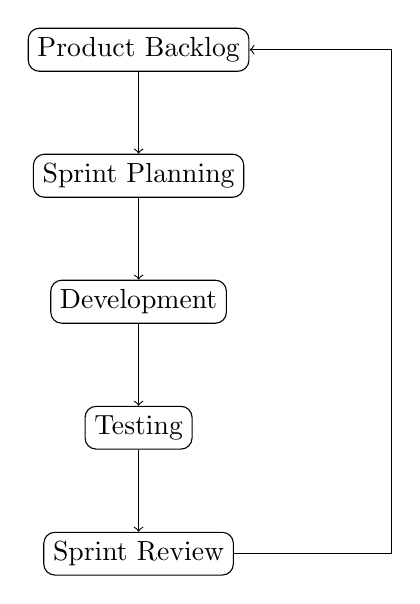
\begin{tikzpicture}[node distance=1.6cm]

\node (backlog) [draw, rectangle, rounded corners] {Product Backlog};
\node (planning) [draw, rectangle, rounded corners, below of=backlog] {Sprint Planning};
\node (development) [draw, rectangle, rounded corners, below of=planning] {Development};
\node (testing) [draw, rectangle, rounded corners, below of=development] {Testing};
\node (review) [draw, rectangle, rounded corners, below of=testing] {Sprint Review};

\draw[->] (backlog) -- (planning);
\draw[->] (planning) -- (development);
\draw[->] (development) -- (testing);
\draw[->] (testing) -- (review);
\draw[->] (review.east) -- ++(2,0) |- (backlog.east);

\end{tikzpicture}
\end{center}

\subsection{Sprint-based Development}

The project execution was divided into four main iterative sprints:
\begin{itemize}
    \item \textbf{Sprint 1 (Foundation):} Setup MERN architecture, Express API server, Mongoose data schemas, and JWT multi-role authentication.
    \item \textbf{Sprint 2 (Core LMS \& Quizzes):} Develop course builder, PDF document upload, section/lesson routes, timed quiz engine, and scoring pipeline.
    \item \textbf{Sprint 3 (AI RAG Subsystem):} Integrate LangChain PDF extraction, OpenAI embedding generation, Pinecone index search, and grounded AI Tutor UI with page badges.
    \item \textbf{Sprint 4 (Personalization & Telemetry):} Implement weak-topic calculation algorithm, AI study plan task generator, dynamic calendar integration, and system documentation.
\end{itemize}

\section{Requirement Analysis}

Requirement analysis establishes the complete software and hardware specifications necessary to build and deploy AI-LMS.

\subsection{Software Requirements}

The primary software stack used in AI-LMS is detailed in Table \ref{tab:sw_req}.

\begin{table}[H]
\centering
\caption{Software Requirements}
\label{tab:sw_req}
\begin{tabular}{p{0.32\textwidth} p{0.58\textwidth}}
\toprule
\textbf{Software / Technology} & \textbf{Purpose} \\
\midrule
React 18.3 & Frontend user interface framework. \\
Vite 5.2 & Fast frontend build and development tool. \\
Tailwind CSS 3.4 & Utility-first responsive CSS styling. \\
React Router 6 & Client-side routing and protected route guards. \\
Node.js v18+ & JavaScript runtime environment for backend API. \\
Express.js 4.19 & RESTful web framework for 14 API route modules. \\
MongoDB Atlas / Mongoose 8.4 & NoSQL document database and ODM modeling. \\
Pinecone Vector DB v3.0 & Dense 1536-dimensional vector similarity search. \\
LangChain TextSplitters v1.0 & PDF document text loader and chunk splitter. \\
OpenAI Node SDK v7.4 & LLM API (\texttt{gpt-4o-mini}) and embeddings (\texttt{text-embedding-3-small}). \\
JWT \& BcryptJS & User authentication and encrypted password storage. \\
Git \& GitHub & Version control and repository management. \\
\bottomrule
\end{tabular}
\end{table}

\subsection{Hardware Requirements}

The hardware specifications for hosting and running the application are outlined in Table \ref{tab:hw_req}.

\begin{table}[H]
\centering
\caption{Hardware Requirements}
\label{tab:hw_req}
\begin{tabular}{p{0.35\textwidth} p{0.55\textwidth}}
\toprule
\textbf{Component} & \textbf{Development Server / Client Spec} \\
\midrule
Processor & Quad-Core Intel i7 / AMD Ryzen 7 / Apple M1+ (Client: Dual-Core 1.6 GHz). \\
RAM & 16 GB DDR4/DDR5 recommended (Client: Minimum 4 GB). \\
Storage & 20 GB NVMe SSD available space. \\
Display & Standard 1080p Monitor or Laptop Display. \\
Network & Broadband Internet connection (50+ Mbps for API calls). \\
\bottomrule
\end{tabular}
\end{table}

\section{Summary}

The system study identified key operational gaps in static LMS platforms and generic AI chatbots, laying the groundwork for AI-LMS. By combining Retrieval-Augmented Generation, vector embeddings, and telemetry-based personalization within a secure MERN framework, AI-LMS delivers a grounded, adaptive digital learning experience. The requirements and sprint methodology defined in this chapter form the basis for the architectural and system design detailed in Chapter 4.
